\documentclass{article}
\usepackage{amsmath,amssymb}
\usepackage{graphicx}
\usepackage{enumerate}
\usepackage{hyperref}
\usepackage{subcaption}
\usepackage{caption}
\usepackage{xcolor}

\pagestyle{empty} \addtolength{\textwidth}{1.0in}
\addtolength{\textheight}{0.5in}
\addtolength{\oddsidemargin}{-0.5in}
\addtolength{\evensidemargin}{-0.5in}
\newcommand{\ruleskip}{\bigskip\hrule\bigskip}
\newcommand{\nodify}[1]{{\sc #1}}
\newcommand{\points}[1]{{\textbf{[#1 points]}}}
\newcommand{\subquestionpoints}[1]{{[#1 points]}}
\newenvironment{answer}{{\bf Answer:} \sf }{}%

\newcommand{\bitem}{\begin{list}{$\bullet$}%
{\setlength{\itemsep}{0pt}\setlength{\topsep}{0pt}%
\setlength{\rightmargin}{0pt}}}
\newcommand{\eitem}{\end{list}}

\setlength{\parindent}{0pt} \setlength{\parskip}{0.5ex}
\setlength{\unitlength}{1cm}

\newcommand{\pa}[1]{[[PA: #1]]}

\renewcommand{\Re}{{\mathbb R}}
\newcommand{\E}{{\rm E}}
\begin{document}

\pagestyle{myheadings} \markboth{}{CS287 Advanced Robotics, Homework \#1, Fall 2019}

{\huge
\noindent Homework \#1: Value Iteration, Discretization}
\ruleskip

{\bf Deliverable}:  PDF write-up by {\bf Wednesday September 18th, 23:59pm}.  Your PDF should be generated by simply replacing the placeholder images of this LaTeX document with the appropriate solution images that will be generated automatically when solving each question.  Your PDF is to be submitted into www.gradescope.com.  Look at the \texttt{README.md} file for running each question and modifying the arguments. This PDF already contains a few solution images.  These images will allow you to check your own solution to ensure correctness.  If any parameters are not specified explicitly, for reporting purposes make sure to use the default settings in the environments.   


\vspace{.2in}

%--------------------------------------------------------------------------------
%--------------------------------------------------------------------------------
%--------------------------------------------------------------------------------
\noindent {\bf 1. Value Iteration}
%--------------------------------------------------------------------------------
%--------------------------------------------------------------------------------
%--------------------------------------------------------------------------------

\begin{enumerate}[(a)]

\item {\bf [15pt] Value iteration.} First, you will implement the value iteration algorithm for the tabular case. You will need to fill the code in \texttt{part1/tabular\_value\_iteration.py} below the lines \texttt{if self.policy\_type == `deterministic'}. Run part 1's run script and report the heatmap of the converged values.

\begin{figure}[h!]
    \centering
    \begin{subfigure}{0.45\textwidth}
        \centering
        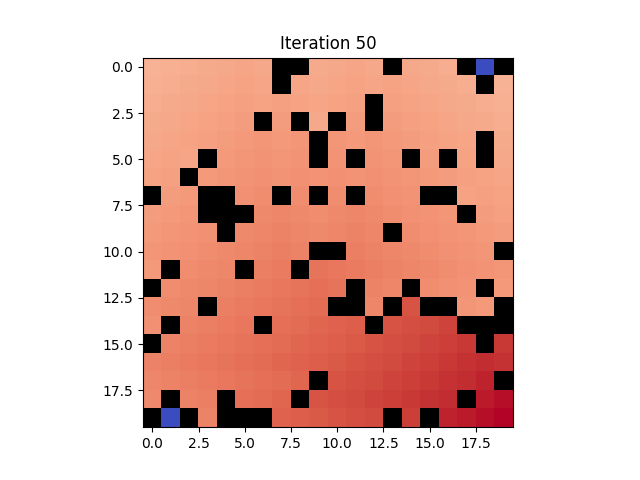
\includegraphics[width=\textwidth]{figures/part_1_a.png}
        \caption{Heatmap of the final values on the \texttt{GridWorld(0)} environment.}
    \end{subfigure}
    \hspace{0.2in}
    \begin{subfigure}{0.45\textwidth}
        \centering
        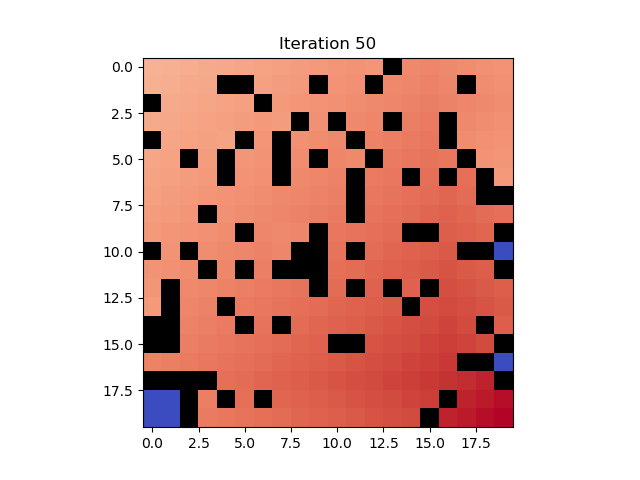
\includegraphics[width=\textwidth]{figures/part_1_a_grid1.png}
        \caption{Heatmap of the final values on the \texttt{GridWorld(1)} environment.  \textcolor{red}{My Solutions}}
    \end{subfigure}
\end{figure}

\newpage 

\item {\bf [15pth] Maxent value iteration.} In cases where the environment might change, a deterministic policy would mostly likely fail. In this scenarios a stochastic policy results more robust. This stochastic policy can be obtained by solving the maximum entropy value iteration.  You will need to fill the code in \texttt{part1/tabular\_value\_iteration.py} below the lines \texttt{if self.policy\_type == `max\_ent'}. Run part 1's run script with the maximum entropy policy and report the heatmap of the converged values for the temperature values $1, 1\text{e-}2, 1\text{e-}5$. In order to stabilize the training: 1) Make sure to add $\texttt{self.eps}$ to the policy's probabilities, and 2) compute the exponentiated values after first subtracting the maximum value across all actions for each state (a standard way to stabilize softmax calculations):
\begin{align*}
    &\pi_k(a|s) = \frac{1}{Z} \left( \text{exp} \left( \frac{1}{\beta}(Q(s, a) - \max_a Q(s, a)) \right) + \epsilon \right) \\
        &V_k(s) = \beta \log \left(\sum_a \text{exp}\left(\frac{1}{\beta}(Q(s, a) - \max_a Q(s, a))\right) \right) + \max_a Q(s, a)
\end{align*}

The $\epsilon$ value prevents the probabilities to be $0$, or close to it, stabilizing the $\log(\pi_k(a|s))$ term of the entropy. Subtracting $\max_a Q(s, a)$ forces all the values in the exponential to be negative preventing large values on the exponential term which would raise numerical problems. Make sure to compute the normalization constant after doing this processing so the probabilities add up to 1.

\begin{figure}[h!]
    \centering
    \begin{subfigure}{0.3\textwidth}
        \centering
        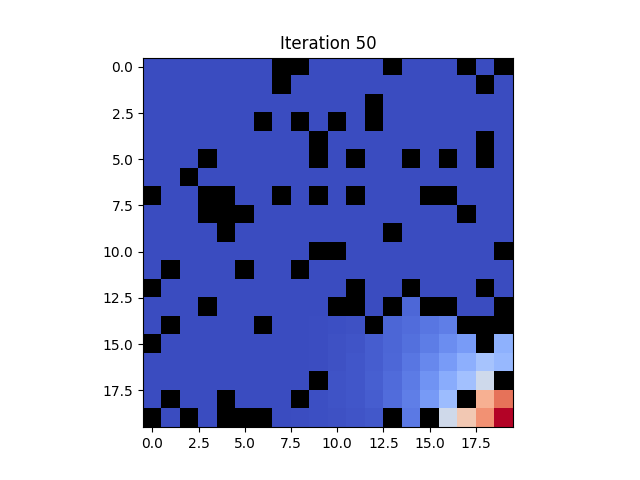
\includegraphics[width=\textwidth]{figures/part_1_b_t1.png}
        \caption{Heatmap of the final values on the \texttt{GridWorld(0)} environment using a maximum entropy policy with temperature equal to 1.}
    \end{subfigure}
    \hspace{0.1 in}
    \begin{subfigure}{0.3\textwidth}
        \centering
        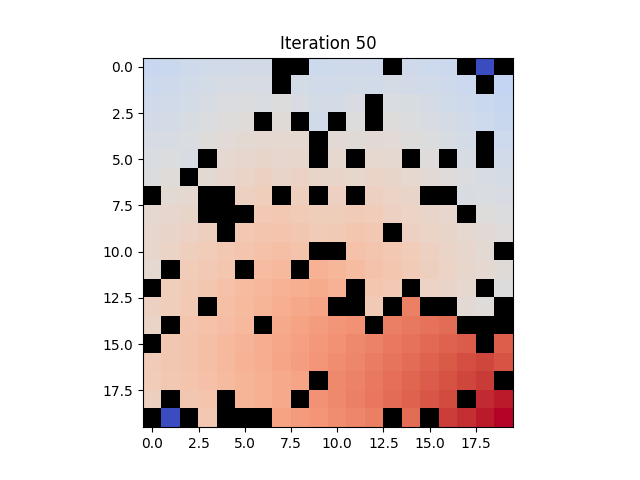
\includegraphics[width=\textwidth]{figures/part_1_b_t1e-2.png}
        \caption{Heatmap of the final values on the \texttt{GridWorld(0)} environment using a maximum entropy policy with temperature equal to 1e-2.}
    \end{subfigure}
    \hspace{0.1 in}
     \begin{subfigure}{0.3\textwidth}
        \centering
        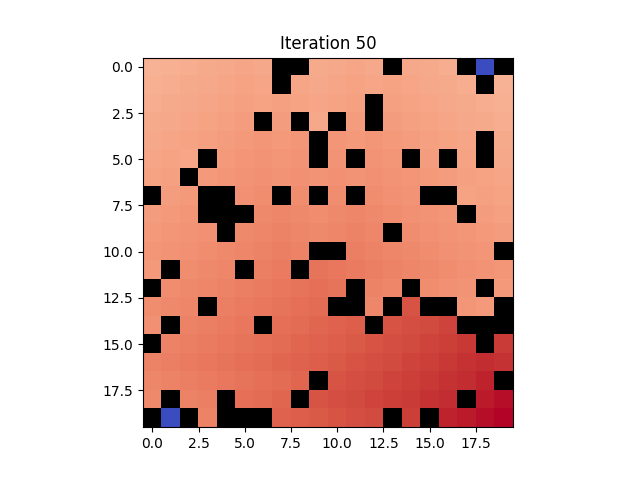
\includegraphics[width=\textwidth]{figures/part_1_b_t1e-5.png}
        \caption{Heatmap of the final values on the \texttt{GridWorld(0)} environment using a maximum entropy policy with temperature equal to 1e-5.}
    \end{subfigure}
\end{figure}
\vspace{-0.1 in}

\begin{figure}[h!]
    \centering
    \begin{subfigure}{0.3\textwidth}
        \centering
        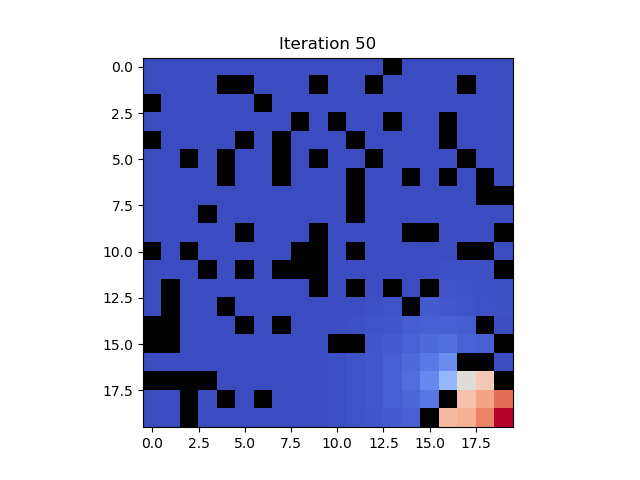
\includegraphics[width=\textwidth]{figures/part_1_b_t1_grid1.png}
        \caption{Heatmap of the final values on the \texttt{GridWorld(1)} environment using a maximum entropy policy with temperature equal to 1.  \textcolor{red}{My Solutions}}
    \end{subfigure}
    \hspace{0.1 in}
    \begin{subfigure}{0.3\textwidth}
        \centering
        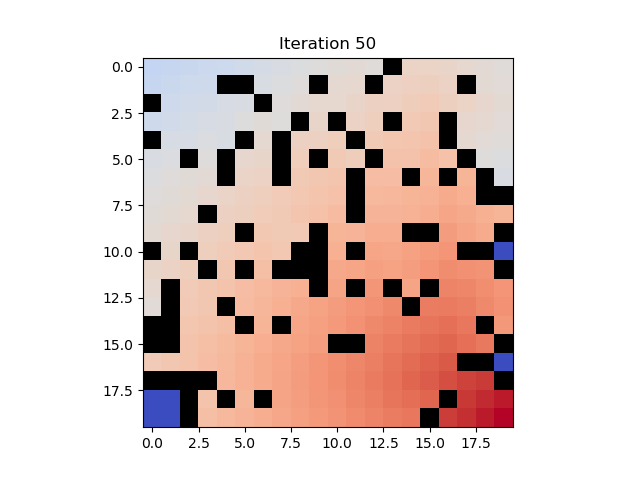
\includegraphics[width=\textwidth]{figures/part_1_b_t1e-2_grid1.png}
        \caption{Heatmap of the final values on the \texttt{GridWorld(1)} environment using a maximum entropy policy with temperature equal to 1e-2.  \textcolor{red}{My Solutions}}
    \end{subfigure}
    \hspace{0.1 in}
     \begin{subfigure}{0.3\textwidth}
        \centering
        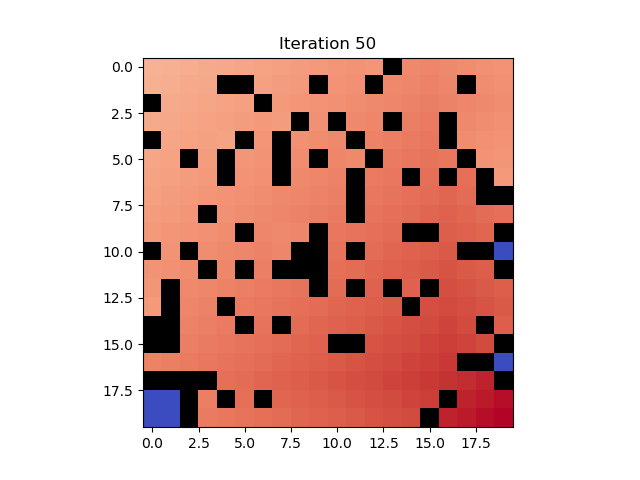
\includegraphics[width=\textwidth]{figures/part_1_b_t1e-5_grid1.png}
        \caption{Heatmap of the final values on the \texttt{GridWorld(1)} environment using a maximum entropy policy with temperature equal to 1e-5.  \textcolor{red}{My Solutions}}
    \end{subfigure}
\end{figure}

\textcolor{red}{I want to try with naive formula without subtracting $\max_a Q(s,a$) or adding $\epsilon$}
\textcolor{red}{
\begin{align*}
	&\pi_k(a|s) = \frac{1}{Z}  \text{exp}  \left(\frac{1}{\beta}Q(s,a) \right)\\
	&V_k(s) = \beta \log \left( \sum_a \text{exp} \left( \frac{1}{\beta}Q_k(s,a) \right)\right)
\end{align*}
}

\begin{figure}[h!]
    \centering
    \begin{subfigure}{0.3\textwidth}
        \centering
        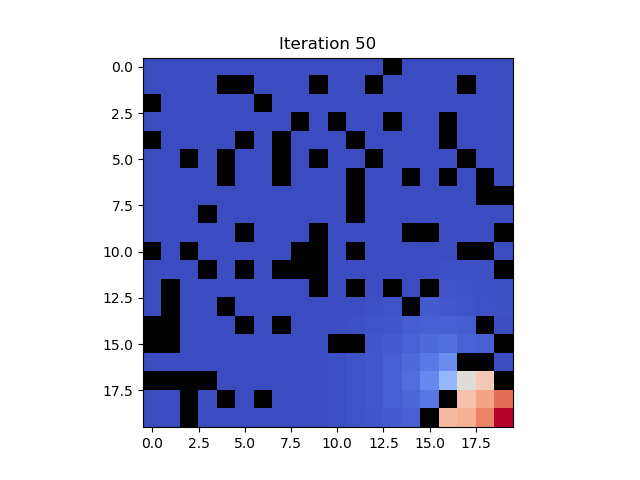
\includegraphics[width=\textwidth]{figures/part_1_b_t1_naive.png}
        \caption{Heatmap of the final values on the \texttt{GridWorld(1)} environment using a maximum entropy policy with temperature equal to 1.  \textcolor{red}{My Solutions}}
    \end{subfigure}
    \hspace{0.1 in}
    \begin{subfigure}{0.3\textwidth}
        \centering
        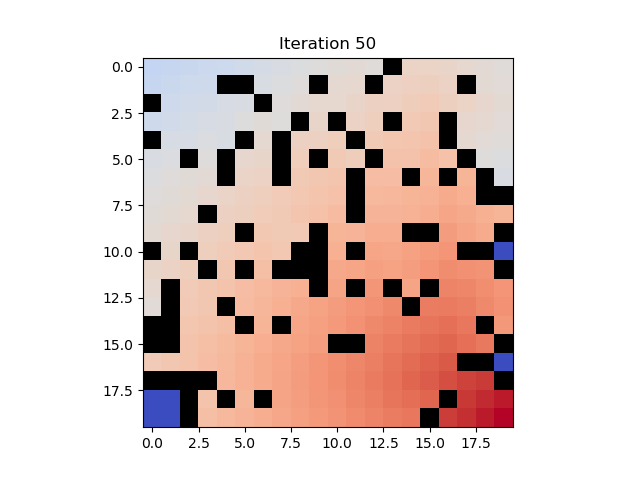
\includegraphics[width=\textwidth]{figures/part_1_b_t0-01_naive.png}
        \caption{Heatmap of the final values on the \texttt{GridWorld(1)} environment using a maximum entropy policy with temperature equal to 1e-2.  \textcolor{red}{My Solutions}}
    \end{subfigure}
    \hspace{0.1 in}
     \begin{subfigure}{0.3\textwidth}
        \centering
        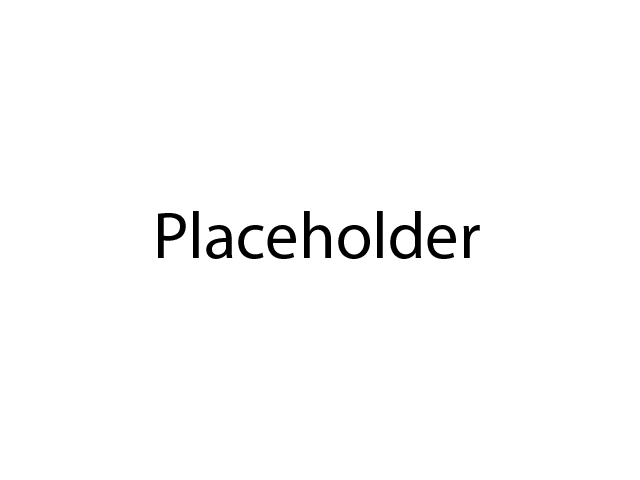
\includegraphics[width=\textwidth]{figures/placeholder.png}
        \caption{Heatmap of the final values on the \texttt{GridWorld(1)} environment using a maximum entropy policy with temperature equal to 1e-5.  \textcolor{red}{Error because nan in solutions, which is due to unstable in exp}}
    \end{subfigure}
\end{figure}


\end{enumerate}



%--------------------------------------------------------------------------------
%--------------------------------------------------------------------------------
%--------------------------------------------------------------------------------
\newpage 
\noindent {\bf 2. Discretization}
%--------------------------------------------------------------------------------
%--------------------------------------------------------------------------------
%--------------------------------------------------------------------------------

\begin{enumerate}[(a)]

\item {\bf [10pt] Nearest-neighbor interpolation.} The value iteration algorithm that you implemented in the last part is just valid when the state space and the action space is discrete. What do we do when we are posed with a problem that has the state space and/or the action space continuous. One solution is to discretize such spaces so the previous algorithm is still valid. In this question, you are asked to implement the more naive discretization scheme: nearest-neighbor interpolation. You will need to fill the code in \texttt{part2/discretize.py} below the lines \texttt{if self.mode == `nn'}. Run part 2's run script and report the heatmap for \texttt{MountainCar} discretizing each dimension of the state space into 21, 51, and 151 bins.

\begin{figure}[h!]
    \centering
    \begin{subfigure}{0.3\textwidth}
        \centering
        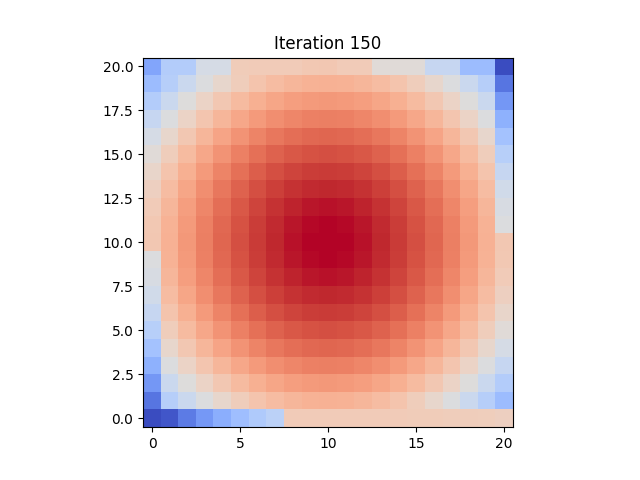
\includegraphics[width=\textwidth]{figures/part_2_a_a.png}
        \caption{Heatmap of the values after 150 iterations of the value iteration algorithm on the \texttt{DoubleIntegrator} environment. 
                The state space is discretized in 21 points and the action space into 5 points using the nearest-neighbor interpolation.}
    \end{subfigure}
    \hspace{0.1 in}
    \begin{subfigure}{0.3\textwidth}
        \centering
        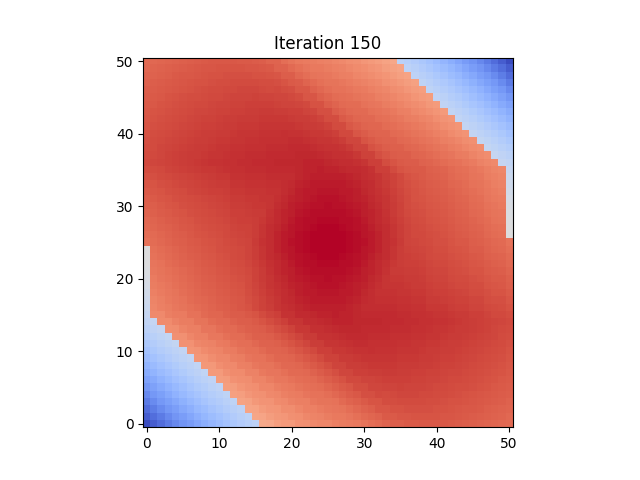
\includegraphics[width=\textwidth]{figures/part_2_a_b.png}
        \caption{Heatmap of the values after 150 iterations of the value iteration algorithm on the \texttt{DoubleIntegrator} environment. 
                The state space is discretized in 51 points and the action space into 5 points using the nearest-neighbor interpolation.}
    \end{subfigure}
        \hspace{0.1 in}
    \begin{subfigure}{0.3\textwidth}
        \centering
        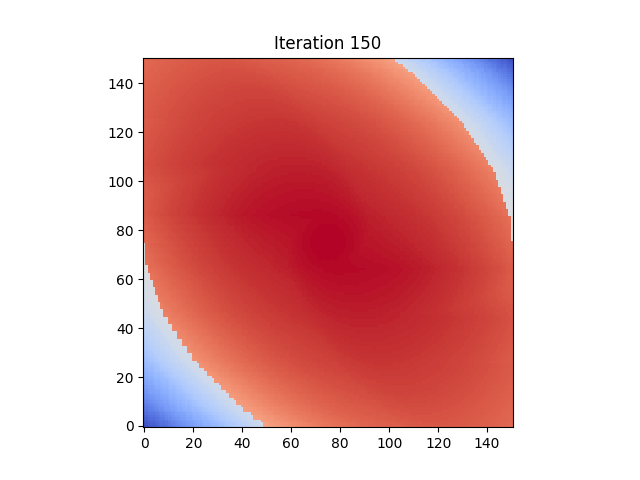
\includegraphics[width=\textwidth]{figures/part_2_a_c.png}
        \caption{Heatmap of the values after 150 iterations of the value iteration algorithm on the \texttt{DoubleIntegrator} environment. 
                The state space is discretized in 151 points and the action space into 5 points using the nearest-neighbor interpolation.}
    \end{subfigure}
    \\
    \centering
    \begin{subfigure}{0.3\textwidth}
        \centering
        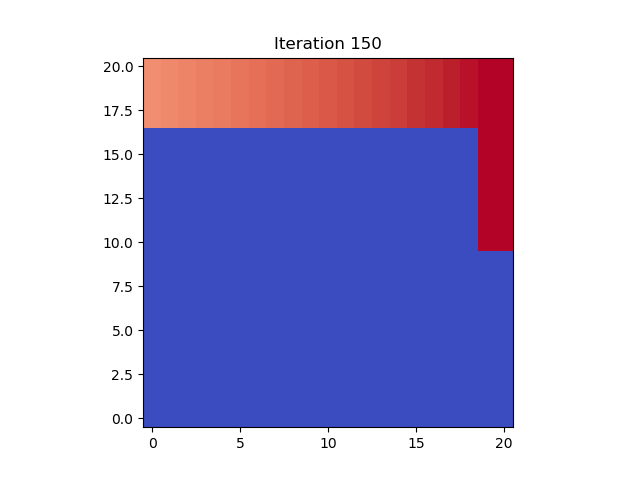
\includegraphics[width=\textwidth]{figures/part_2_moutain-car_s-21.png}
\caption{Heatmap of the values after 150 iterations of the value iteration algorithm on the \texttt{MountainCar} environment. 
                The state space is discretized in 21 points using the nearest-neighbor interpolation.}
    \end{subfigure}
    \hspace{0.1 in}
    \begin{subfigure}{0.3\textwidth}
        \centering
        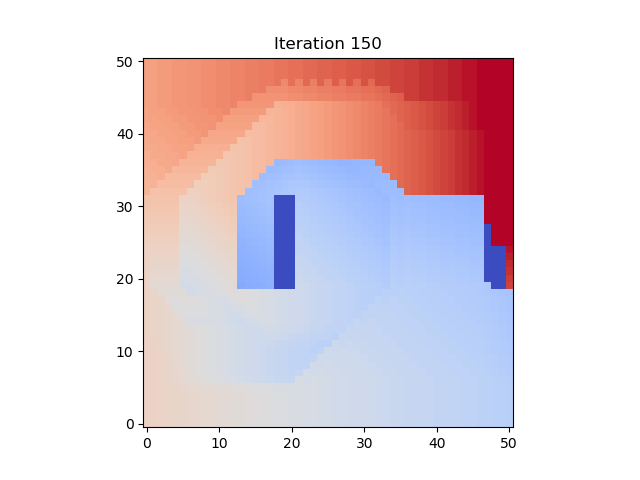
\includegraphics[width=\textwidth]{figures/part_2_moutain-car_s-51.png}
\caption{Heatmap of the values after 150 iterations of the value iteration algorithm on the \texttt{MountainCar} environment. 
                The state space is discretized in 51 points using the nearest-neighbor interpolation.}
    \end{subfigure}
        \hspace{0.1 in}
    \begin{subfigure}{0.3\textwidth}
        \centering
        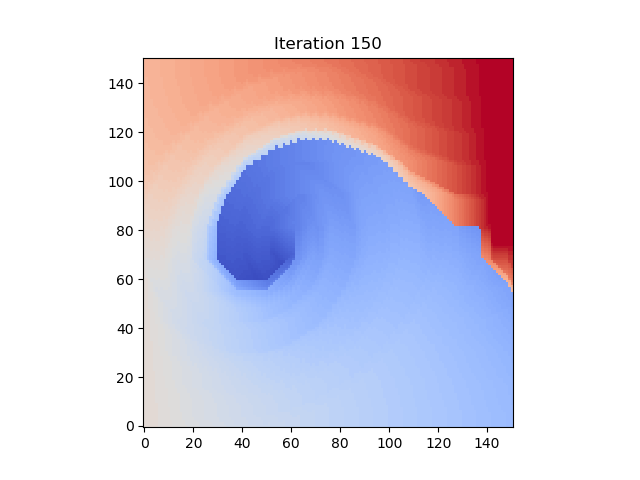
\includegraphics[width=\textwidth]{figures/part_2_moutain-car_s-151.png}
\caption{Heatmap of the values after 150 iterations of the value iteration algorithm on the \texttt{MountainCar} environment. 
                The state space is discretized in 151 points using the nearest-neighbor interpolation.}
    \end{subfigure}
\end{figure}

\newpage
\item {\bf [10pt] n-linear interpolation.} Discretization using nearest-neighbors is able to recover the optimal solution if your discretization is fine enough. However, the number of points increase exponentially with the dimensionality of your problem. The naive scheme of nearest-neighbors is not computationally tractable for higher dimensional problems. In this question, you will implement a better discretization scheme: n-linear interpolation, the analogous of linear interpolation in n dimensions. To do so, you will need to fill the code in \texttt{part2/discretize.py} below the lines \texttt{if self.mode == `linear'}. Run part 2's run script and report the heatmap for \texttt{MountainCar} for different discretization resolution: 21, 51, and 151 points per dimension.

\begin{figure}[h!]
    \centering
    \begin{subfigure}{0.3\textwidth}
        \centering
        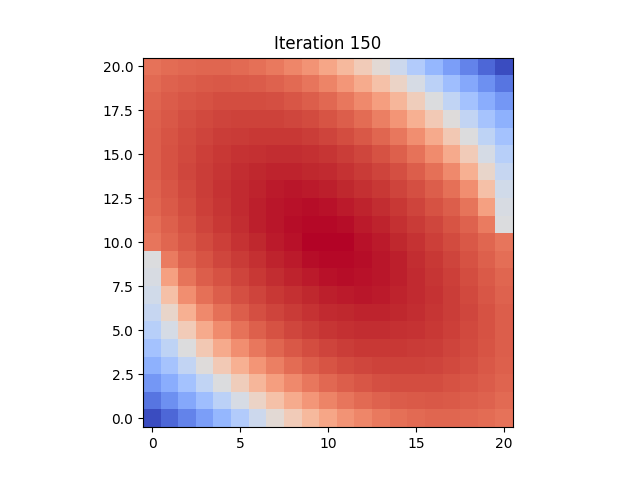
\includegraphics[width=\textwidth]{figures/part_2_b_a.png}
        \caption{Heatmap of the values after 150 iterations of the value iteration algorithm on the \texttt{DoubleIntegrator} environment. 
                The state space is discretized in 21 points and the action space into 5 points using the n-linear interpolation.}
    \end{subfigure}
    \hspace{0.1 in}
    \begin{subfigure}{0.3\textwidth}
        \centering
        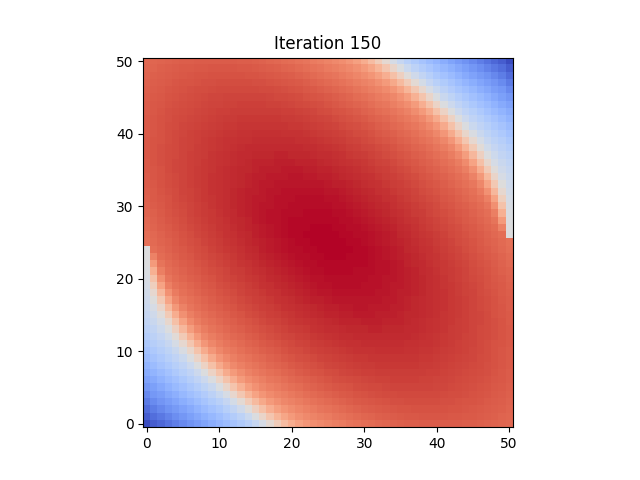
\includegraphics[width=\textwidth]{figures/part_2_b_b.png}
        \caption{Heatmap of the values after 150 iterations of the value iteration algorithm on the \texttt{DoubleIntegrator} environment. 
                The state space is discretized in 51 points and the action space into 5 points using the n-linear interpolation.}
    \end{subfigure}
    \hspace{0.1 in}
    \begin{subfigure}{0.3\textwidth}
        \centering
        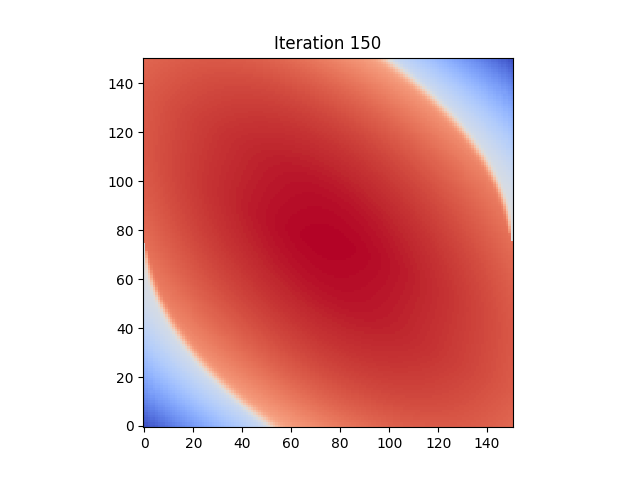
\includegraphics[width=\textwidth]{figures/part_2_b_c.png}
        \caption{Heatmap of the values after 150 iterations of the value iteration algorithm on the \texttt{DoubleIntegrator} environment. 
                The state space is discretized in 151 points and the action space into 5 points using the n-linear interpolation.}
    \end{subfigure}
    \\
    \centering
    \begin{subfigure}{0.3\textwidth}
        \centering
        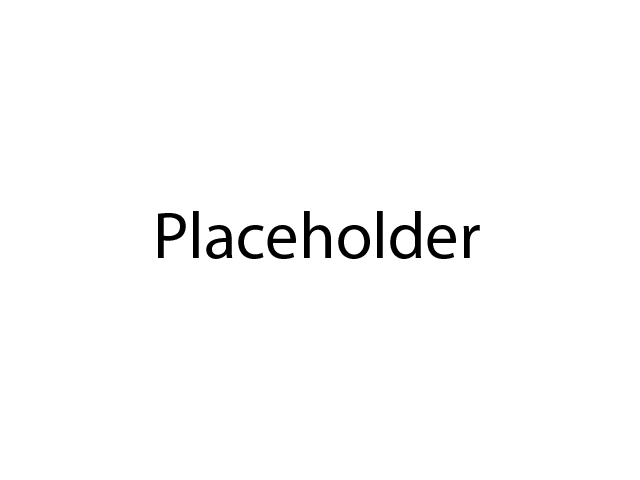
\includegraphics[width=\textwidth]{figures/placeholder.png}
\caption{Heatmap of the values after 150 iterations of the value iteration algorithm on the \texttt{MountainCar} environment. 
                The state space is discretized in 21 points using the n-linear interpolation.}
    \end{subfigure}
    \hspace{0.1 in}
    \begin{subfigure}{0.3\textwidth}
        \centering
        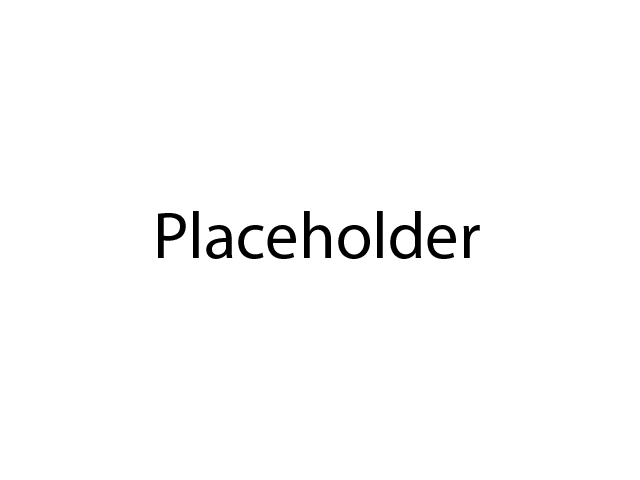
\includegraphics[width=\textwidth]{figures/placeholder.png}
\caption{Heatmap of the values after 150 iterations of the value iteration algorithm on the \texttt{MountainCar} environment. 
                The state space is discretized in 51 points using the n-linear interpolation.}
                
    \end{subfigure}
        \hspace{0.1 in}
    \begin{subfigure}{0.3\textwidth}
        \centering
        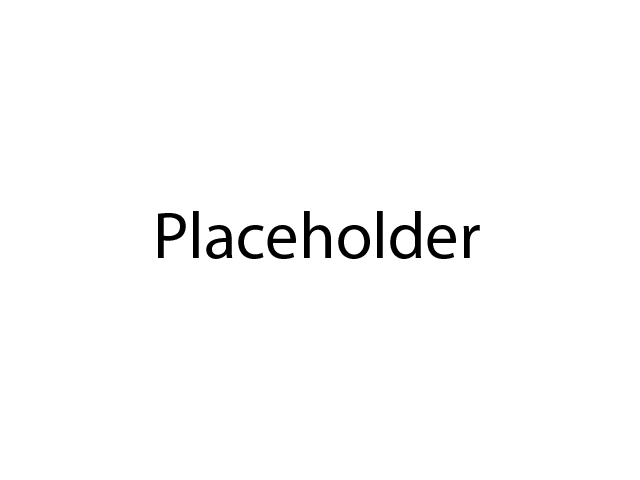
\includegraphics[width=\textwidth]{figures/placeholder.png}
\caption{Heatmap of the values after 150 iterations of the value iteration algorithm on the \texttt{MountainCar} environment. 
                The state space is discretized in 151 points using the n-linear interpolation.}
    \end{subfigure}
\end{figure}

\newpage
\item {\bf [10pt] Nearest-neighbor vs. n-linear interpolation.} Here we will properly compare the performance of both discretization schemes. Specifically, we will compare the average return across iterations for both methods using the same number of points, 21 in this question. You will report the learning curve for the environments \texttt{MountainCar}, \texttt{CartPole}, and \texttt{SwingUp}. As in the example, create different plots for each environment and split the learning curves by discretization scheme. See the \texttt{README.md} file for how to do that.

\begin{figure}[h!]
    \centering
    \begin{subfigure}{0.45\textwidth}
        \centering
        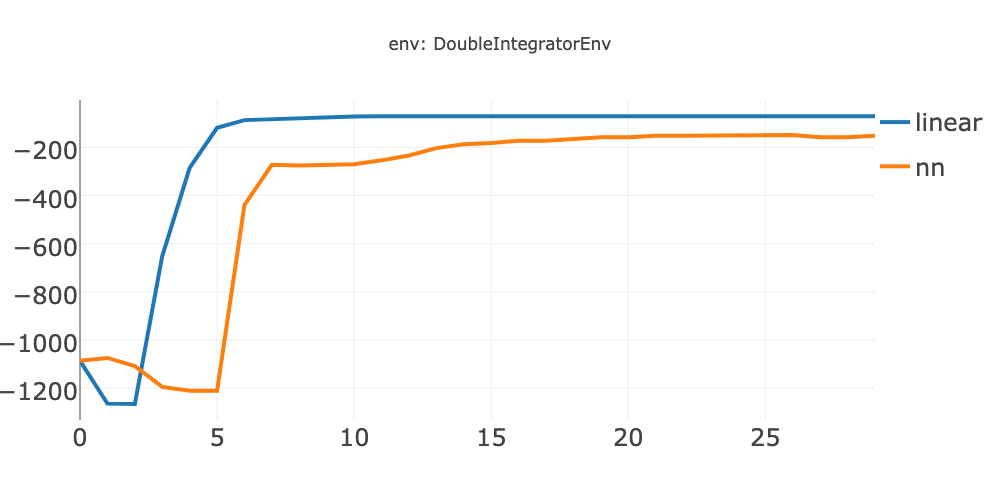
\includegraphics[width=\textwidth]{figures/part_2_c_a.png}
        \caption{Learning curve of  nearest-neighbor and n-linear interpolation in the \texttt{DoubleIntegrator} environment. 
                 The state space is discretized in 151 points and the action space using 5 points.}
    \end{subfigure}
    \hspace{0.2in}
    \begin{subfigure}{0.45\textwidth}
        \centering
        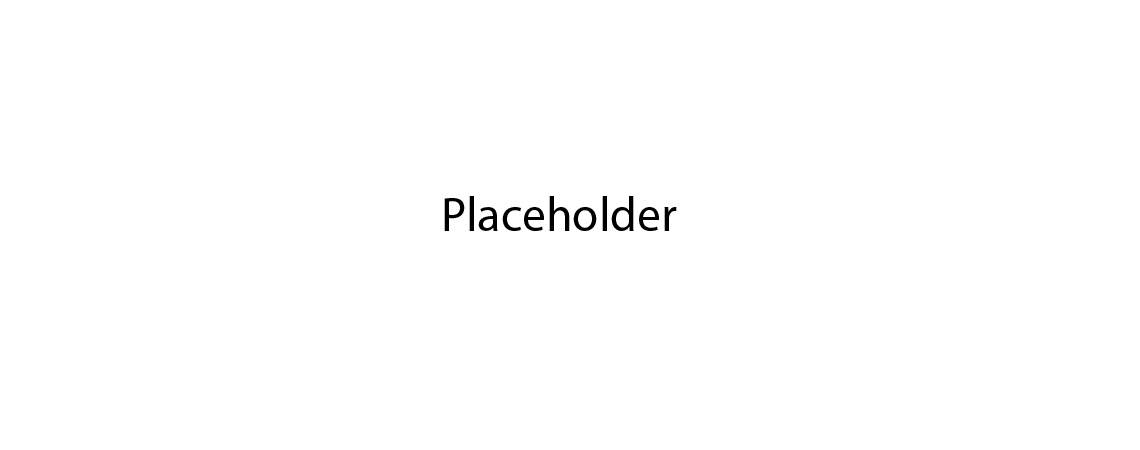
\includegraphics[width=\textwidth]{figures/placeholder_2.png}
         \caption{Learning curve of  nearest-neighbor and n-linear interpolation in the \texttt{MountainCar} environment. 
                 The state space is discretized in 151 points.}
    \end{subfigure}
\\
    \centering
    \begin{subfigure}{0.45\textwidth}
        \centering
        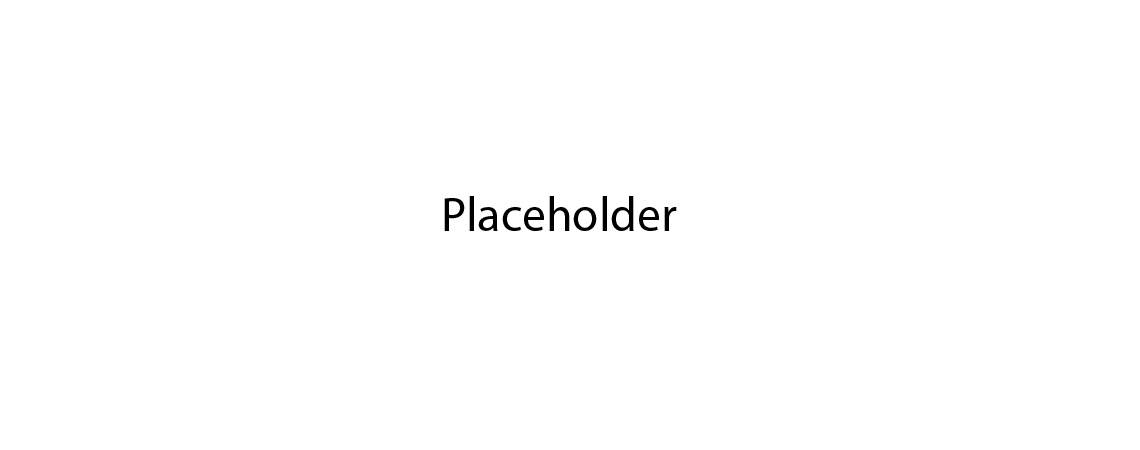
\includegraphics[width=\textwidth]{figures/placeholder_2.png}
        \caption{Learning curve of  nearest-neighbor and n-linear interpolation in the \texttt{CartPole} environment. 
                 The state space is discretized in 21 points.}
    \end{subfigure}
    \hspace{0.2in}
    \begin{subfigure}{0.45\textwidth}
        \centering
        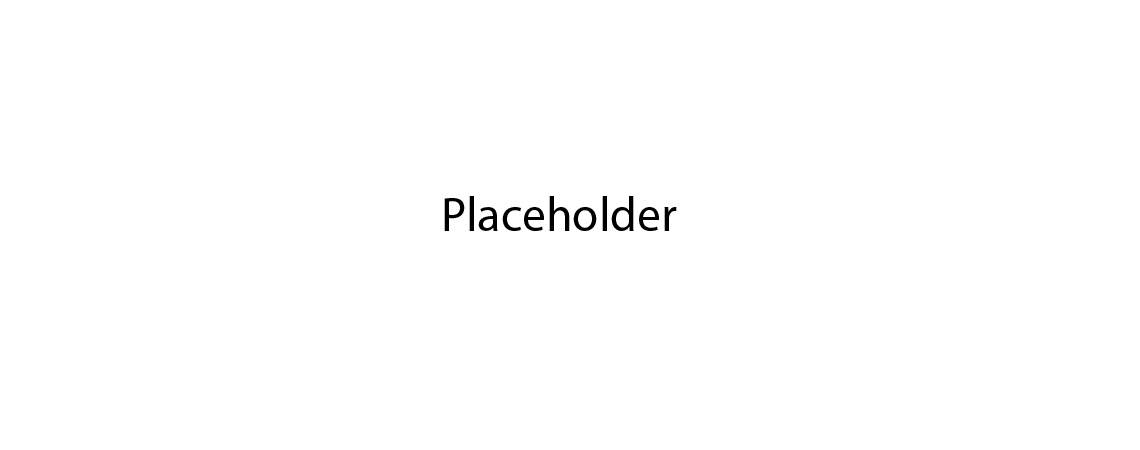
\includegraphics[width=\textwidth]{figures/placeholder_2.png}
          \caption{Learning curve of  nearest-neighbor and n-linear interpolation in the \texttt{SwingUp} environment. 
                 The state space is discretized in 21 points.}
    \end{subfigure}
\end{figure}

\newpage

\item {\bf [15pt] Look-ahead policies.} Value iteration computes the optimal returns for every position in the state space, however it is often the case that we will just need a good policy in a smaller region of the state space. In such case, running value iteration until convergence might seem a waste of resources. Instead, what we can do is to is to run value iteration with a coarser discretization or not until convergence, and then compensate for that by using look-ahead.  In look-ahead we optimize over the first $k$ actions, where we optimize for the sum of near-term reward plus the value achieved in the state achieved after $k$ steps.  In this case, the value achieved will be approximated by the discretization.  After having found the sequence of $k$ actions, the first one is executed, and then the process is repeated.  In this question, we ask you to implement a look-ahead policy. To do so, you will need to fill the code in \texttt{part2/look\_ahead\_policy.py}. Report the learning curves for the values of look ahead horizon equals to 1, 2, and 3 for the \texttt{MountainCar}, \texttt{CartPole}, and \texttt{SwingUp} environment. The results should be split by environment.

\end{enumerate}

\begin{figure}[h!]
    \centering
    \begin{subfigure}{0.45\textwidth}
        \centering
        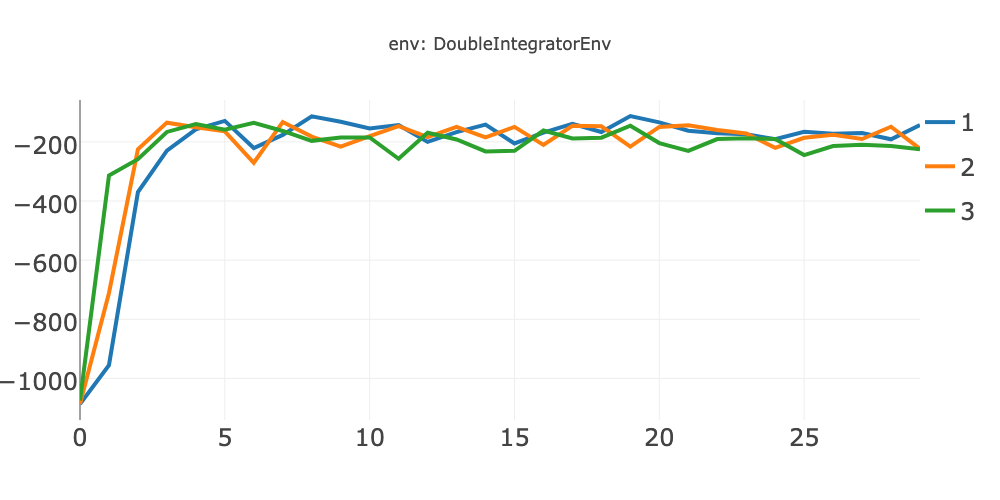
\includegraphics[width=\textwidth]{figures/part_2_d_a.png}
        \caption{Learning curve for different look-ahead horizons in the \texttt{DoubleIntegrator} environment.}
    \end{subfigure}
    \hspace{0.2 in}
    \begin{subfigure}{0.45\textwidth}
        \centering
        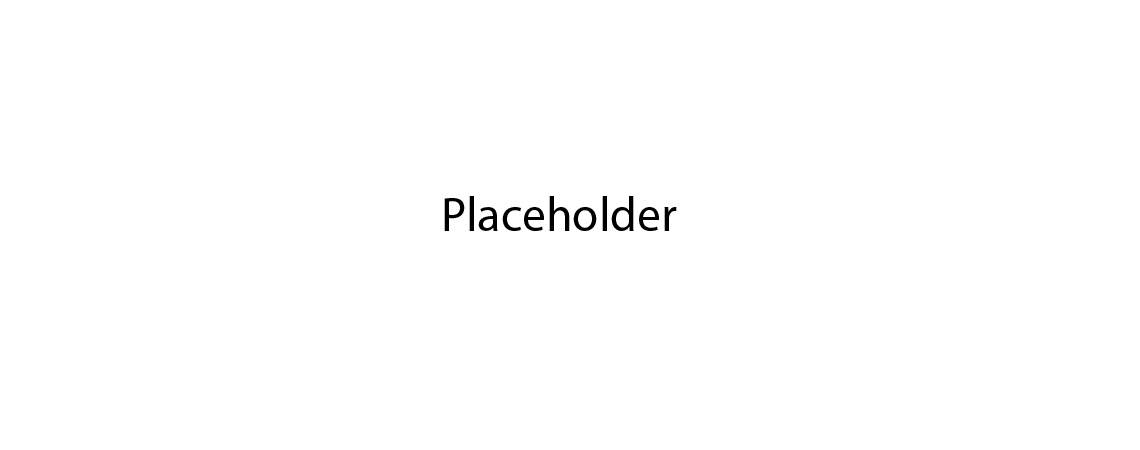
\includegraphics[width=\textwidth]{figures/placeholder_2.png}
        \caption{Learning curve for different look-ahead horizons in the \texttt{MountainCar} environment.}
    \end{subfigure}
\\
    \centering
    \begin{subfigure}{0.45\textwidth}
        \centering
        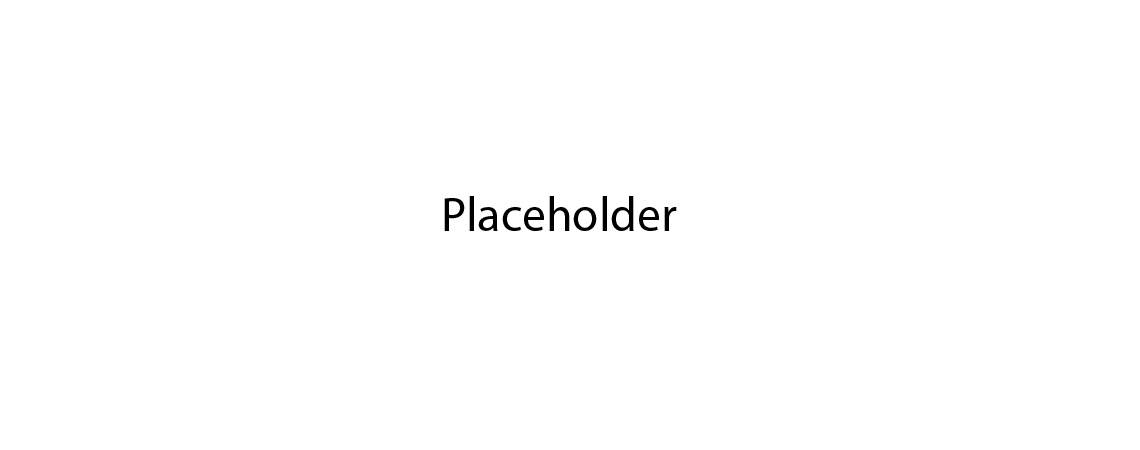
\includegraphics[width=\textwidth]{figures/placeholder_2.png}
        \caption{Learning curve for different look-ahead horizons in the \texttt{CartPole} environment.}
    \end{subfigure}
    \hspace{0.2 in}
    \begin{subfigure}{0.45\textwidth}
        \centering
        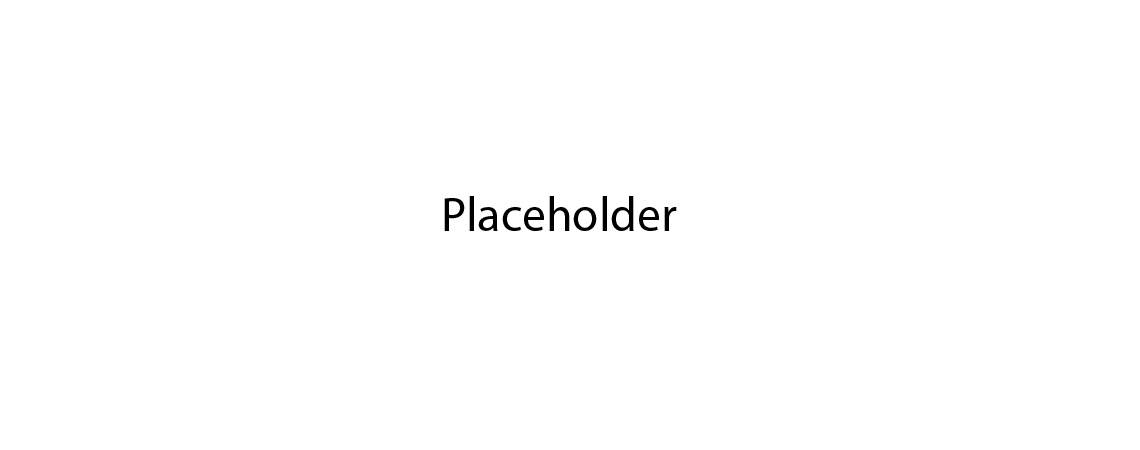
\includegraphics[width=\textwidth]{figures/placeholder_2.png}
        \caption{Learning curve for different look-ahead horizons in the \texttt{SwingUp} environment.}
    \end{subfigure}
\end{figure}

\newpage 
%--------------------------------------------------------------------------------
%--------------------------------------------------------------------------------
%--------------------------------------------------------------------------------
\newpage
\noindent {\bf 3. Value Iteration \& Function Approximation}
%--------------------------------------------------------------------------------
%--------------------------------------------------------------------------------
%--------------------------------------------------------------------------------

\begin{enumerate}[(a)]

\item {\bf [15pt] Value iteration for continuous state spaces.} In higher dimensional domains discretization its unfeasible, since you end up with an exponential number of points. For instance, consider an environment with 10 state dimensions and 5 action dimensions; if we were to discretize each dimension in just 10 points our transition matrix wold ocupy over 1 million GB!! A solution to this problem is to use function approximators: a function parametrize with some set of parameters $\theta$ that maps from states to values. In this excersise we will use a neural network as function approximator (but you can treat it as a black box function). Here, we ask you to implement the value iteration algorithm for function approximators. You will need to fill the code in \texttt{part3/continuous\_value\_iteration.py} and \texttt{part3/look\_ahead\_policy.py}. You will implement a policy that will choose actions by maximizing the value function over a random sample of possible actions. You will need to do it for continuous and discrete actions. Run part 3's run script and report the heatmap for \texttt{MountainCar}.

\begin{figure}[h!]
    \centering
    \begin{subfigure}{0.45\textwidth}
        \centering
        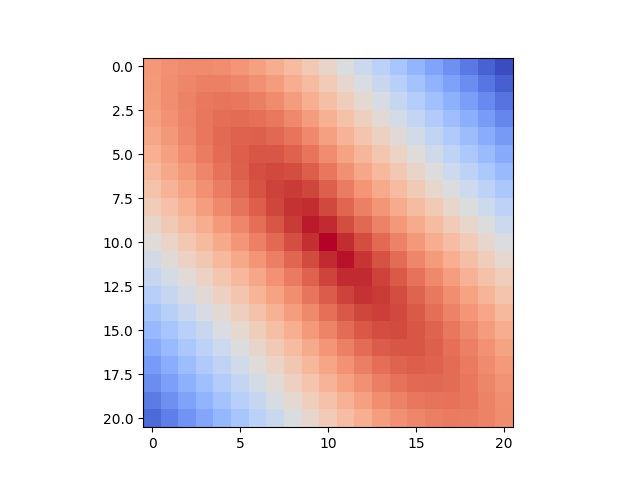
\includegraphics[width=\textwidth]{figures/part_3_a_a.png}
        \caption{Double Integrator}
    \end{subfigure}
    \hspace{0.2 in}
    \begin{subfigure}{0.45\textwidth}
        \centering
        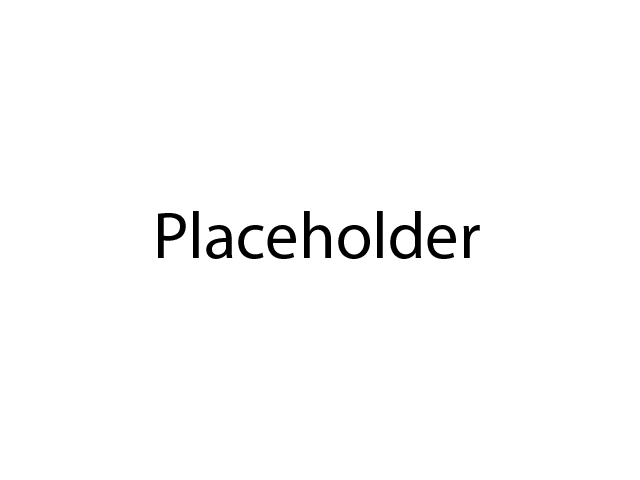
\includegraphics[width=\textwidth]{figures/placeholder.png}
        \caption{Double Integrator}
    \end{subfigure}
\end{figure}

\newpage

\item {\bf [10pt] Look-ahead with cross-entropy for continuous and discrete action spaces.} A better version of the policy implemented before is using look-ahead with cross-entropy method, specially in larger action spaces. You will need to fill the code in \texttt{part3/look\_ahead\_policy.py}. Report the learning curves for look ahead horizon equals to 1, 5, and 10 for all the environments using the cross-entropy method and horizon equals 1 with random shooting. The results should be split by environment.

\begin{figure}[h!]
    \centering
    \begin{subfigure}{0.45\textwidth}
        \centering
        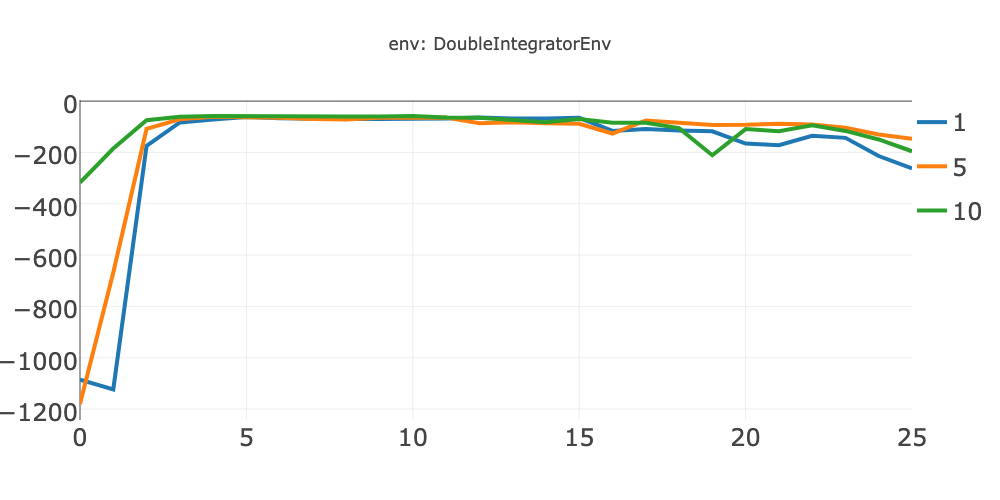
\includegraphics[width=\textwidth]{figures/part_3_b_a.png}
          \caption{Learning curve for different horizons of look ahead on the \texttt{DoubleIntegrator} environment using cross-entropy method for action selection with value function approximation.}
    \end{subfigure}
    \hspace{0.2in}
    \begin{subfigure}{0.45\textwidth}
        \centering
        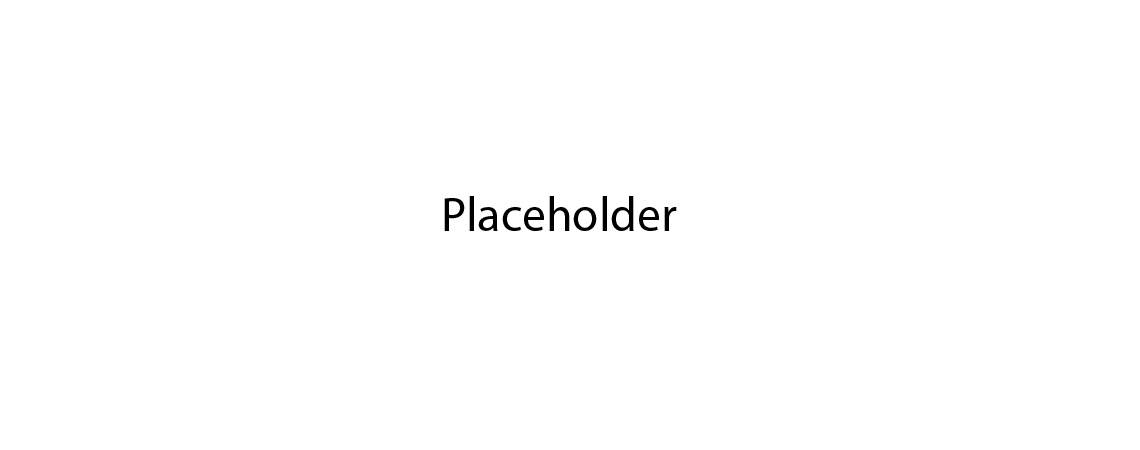
\includegraphics[width=\textwidth]{figures/placeholder_2.png}
         \caption{Learning curve for different horizons of look ahead on the \texttt{MountainCar} environment
                using cross-entropy method for action selection with value function approximation.}
    \end{subfigure}
\\
    \centering
    \begin{subfigure}{0.45\textwidth}
        \centering
        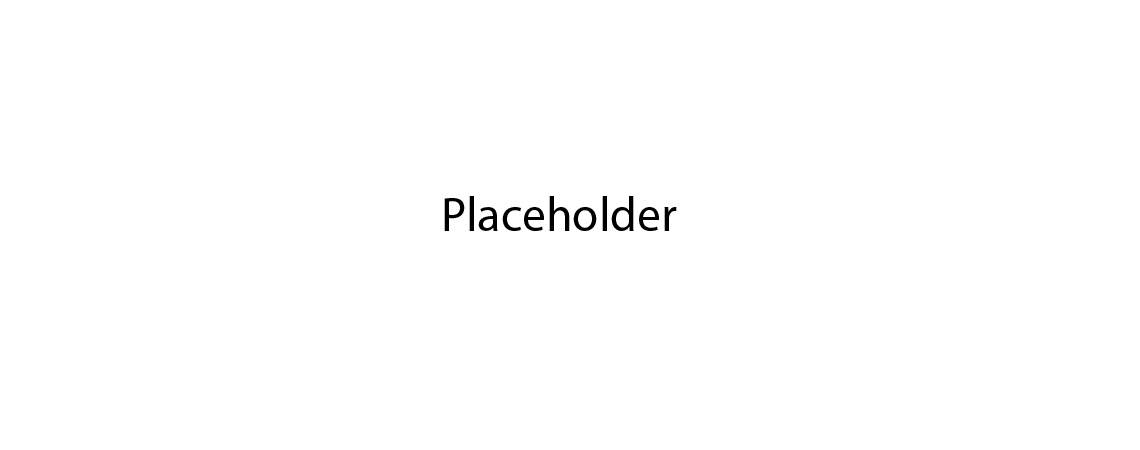
\includegraphics[width=\textwidth]{figures/placeholder_2.png}
          \caption{Learning curve for different horizons of look ahead on the \texttt{CartPole} environment. 
                 using cross-entropy method for action selection with value function approximation.}
    \end{subfigure}
    \hspace{0.2in}
    \begin{subfigure}{0.45\textwidth}
        \centering
        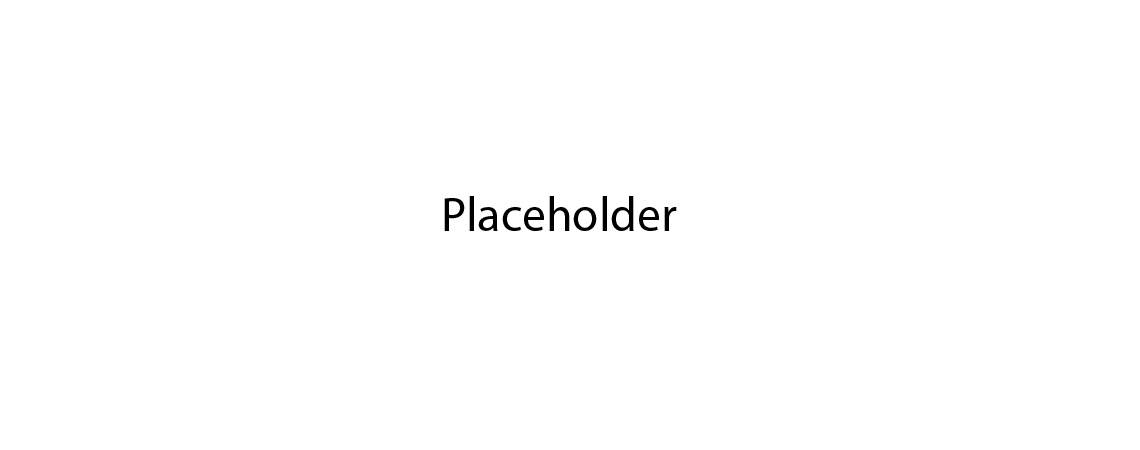
\includegraphics[width=\textwidth]{figures/placeholder_2.png}
          \caption{Learning curve for different horizons of look ahead on the \texttt{SwingUp} environment. 
                 using cross-entropy method for action selection with value function approximation.}
    \end{subfigure}
\end{figure}


\end{enumerate}

\newpage
\noindent {\bf 4. [20pt] Extra Credit: Vectorized Discretization}

As you might have experienced in the \texttt{CartPole} or \texttt{SwingUp} environments, discretization can be pretty slow and just discretizing 21 points might not be enough to achieve learning even with n-linear interpolation (as in the case of \texttt{SwingUp}). The current implementation uses \texttt{for} loops to compute the transition and reward matrix and the discretization the discretization. As extra credit you are asked to implement a vectorized version of part 2.a and achieve maximum performance on \texttt{CartPole} and \texttt{SwingUp} using n-linear interpolation and dicretizing each dimension of the state space in 51 points.

\begin{figure}[h!]
\centering
    \begin{subfigure}{0.45\textwidth}
        \centering
        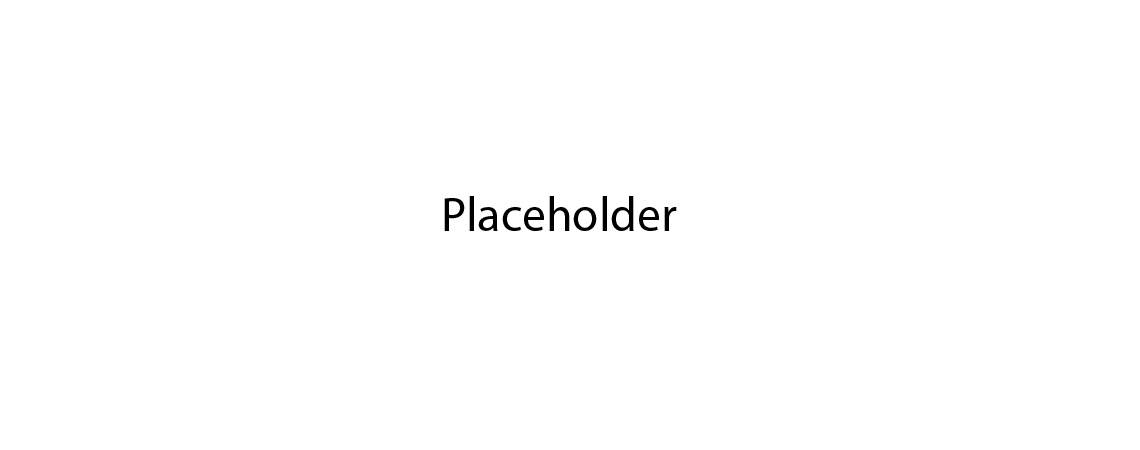
\includegraphics[width=\textwidth]{figures/placeholder_2.png}
          \caption{Learning curve for the \texttt{CartPole} environment.}
    \end{subfigure}
    \hspace{0.2in}
    \begin{subfigure}{0.45\textwidth}
        \centering
        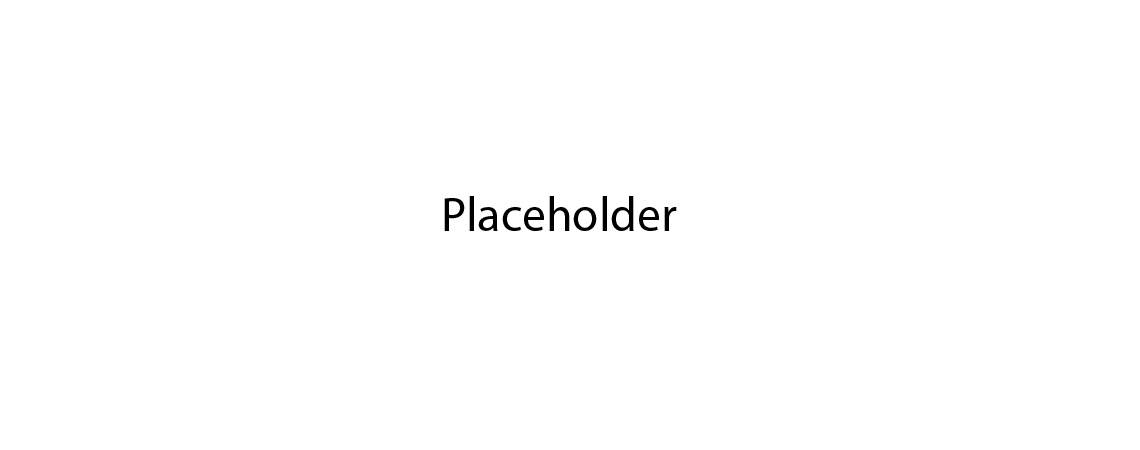
\includegraphics[width=\textwidth]{figures/placeholder_2.png}
          \caption{Learning curve on the \texttt{SwingUp} environment.}
\end{subfigure}
\end{figure}



\end{document}
